\chapter{Related Work}
\label{sec:Related Work}
% This chapter introduces some foundational work on density-based and subspace/correlation clustering and aims to give an intuitive insight into existing approaches to solve the problem of subspace clustering. We also elaborate, where these existing approaches lack in ability and capability and show some of the current optimization approaches.
This chapter introduces some foundational work on subspace/correlation clustering and aims to give an intuitive insight into existing approaches to solve the problem of subspace clustering. In particular the elaboration on the related work is twofold: we introduce subspace/correlation extraction/clustering methods such as basic \acrshort{pca} and \acrshort{orclus}, and additionally expand on algorithms which augment the subspace clustering method such as \acrshort{dbscan} in \acrshort{4c}. We also elaborate, where these existing approaches lack in ability and capability and show some of the current optimization approaches.

Since sections \nameref{sec:houghintro}, \nameref{sec:cashintro}, \nameref{sec:dbscanintro} and \nameref{sec:OPTICSintro} are essential components to our work they will be elaborated in greater detail in the chapter \nameref{sec:Foundations}

\section{Existing Subspace Clustering Algorithms}
There are many approaches for detecting relevant subspaces in data, generally grouped to either finding axis-parallel or arbitrarily oriented subspaces. Our work in particular focuses on the extraction of the second type of subspaces, which obviously proves to be a more challenging task since it encompasses the problem of axis-parallel subspace clustering\todor{the first type}. This task is also referred to as \textit{Correlation Clustering}. 

This section introduces some existing correlation clustering algorithms and illustrates \todor{choose one: demonstrates/analyzes/explains/illustrates/points out} their advantages and disadvantages and elaborates on their suitability for our idea.

\subsection{PCA}
A common way to filter out relevant features/subspaces in high dimensional data is the application of feature selection/dimensionality reduction. One of the oldest and most widely used methods is the \gls{pca}. It is a statistical approach which uses an orthogonal transformation to transform the original basis of a $d$-dimensional data space $DS$ to a basis built upon $d$ so called \textit{Principal Components} $PC$, where the first Principal Components $PC_1$ is a vector which describes the largest percentage of explained variance in $DS$. Each Principal Component $PC_j$ next in order $j,\dotsc,d$ is orthogonal to the previous ones $PC_i, i<j$ and is ordered by the next highest explained variance. Mathematically finding the Principal Components in a data set $DS$ boils down to solving its eigendecomposition \todor{nicht ganz korrekt. eigendecomp von cov(x)}, where the eigenvector with the highest corresponding eigenvalue represents the first Principal Component and the second highest the second Principal Component, etc\cite{pcawold1987principal}. For further details to the calculation \textcite{pcamljolliffe1986principal} offers a short and intuitive step-by-step explanation.
Unfortunately the extraction of relevant features via \gls{pca} is rarely of use for clustering problems. Unmodified \gls{pca} is global in nature and can only compute one subspace of the original data space and does not address the problem of \textit{local feature relevance} or \textit{local feature correlation}, which essentially states, that different clusters in data space can exist in different subspaces\cite{kriegel2009clustering} (c.f. \cite{PCAshlens2014tutorial}). \todor{PCA besser erklaeren}

\todob{PCA own fig}
\begin{figure}
    \centering
    \begin{minipage}[t]{.5\textwidth}
      \centering  
      \captionsetup{width=.9\linewidth}
      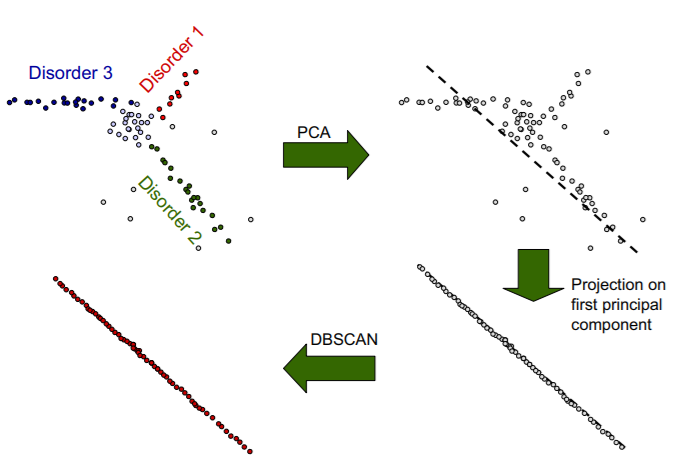
\includegraphics[width=.9\textwidth]{figures/pcalocalfeat1.png}
      \captionof*{figure}{a) First}
      \label{fig:test1}
    \end{minipage}%
    \begin{minipage}[t]{.5\textwidth}
      \centering
      \captionsetup{width=.9\linewidth}
      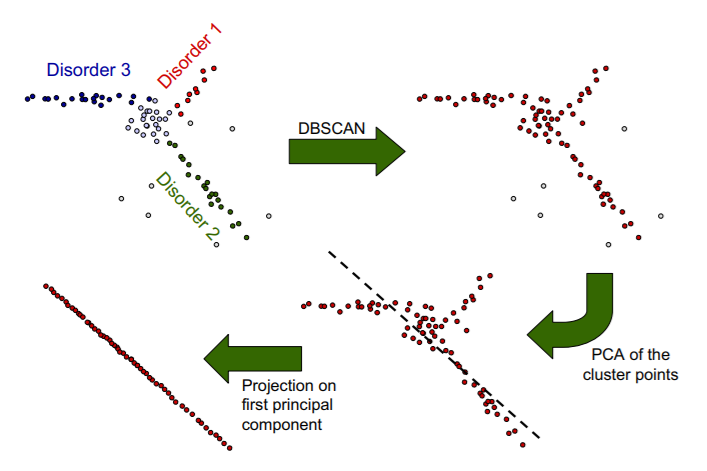
\includegraphics[width=.9\textwidth]{figures/pcalocalfeat2.png}
      \captionof*{figure}{b) Second}
      \label{fig:test2}
    \end{minipage}
    \caption{lazy}
    \label{fig:localfeatrelevance}
\end{figure}

\subsection{ORCLUS}
Since \gls{pca} only provides a global view of the correlations in data space and does not address the local feature relevance, \gls{orclus} attempts to enforce \gls{pca} to only consider local segments of the data space via a $k$-Means-like approach. 

To find $k$ many $l$-dimensional subspace clusters in a $d$-dimensional data space, \gls{orclus} first initializes $k_c, k_c > k$ seeds $s_i$ as centroids and applies the default (euclidean) $k$-Means to partition the data space into $k_c$ clusters $C_i$ with $i \in \{1,\dotsc,k_c\}$. After that iteratively all points are reassigned to the new cluster centroids via a modified distance function based on a subset of $l_c, l\leq l_c \leq d$ weak eigenvectors/principal components $\varepsilon_i$ of each cluster $c_i$. This subset of $l_c$ eigenvectors represents the current dimensionality of the cluster in each iteration and is adapted such that at the end of all iterations $l_c=l$ holds. Additionally at the end of each iteration the closest pair (in terms of average modified distance) of clusters are merged together resulting in $k_c = k_c-1$ clusters afterwards. This reassigning-merging process is repeated until $k_c = k$ holds. Due to the localized view on the single partitions \gls{orclus} is considered as a local correlation clustering algorithm\cite{orclusaggarwal2000finding}.

As an adopter of $k$-Means and \gls{pca}, \gls{orclus} however also comes with its components disadvantages. It relies on $k$, which is difficult to determine, does not handle noise and outliers, and extracts the subspaces based on the clusters eigenvectors, which are not necessarily a good representation of the members distribution (c.f. \autoref{fig:localfeatrelevance}).


\subsection{4C}\label{ssec:4c}
Analogous to \gls{orclus}, \gls{4c} also aims to construct a localized view of the data space. This time however a density-based approach is used. 

To find $\lambda$-dimensional subspace clusters in a $d$-dimensional space, \gls{4c} employs a customized/an extended \acrshort{dbscan} by modifying parts of the density criterion. 
% After clustering the data space into usual dense clusters, each cluster is reevaluated according to its variance. This is done by applying \gls{pca} to the locally dense cluster. If the $d-\lambda$ smallest eigenvectors of the cluster are not close enough to threshold $\delta \approx 0$
Instead of uniformly assessing the neighborhood in all directions, the modified density criterion biases the neighborhood query according to the neighborhoods variance. First, only dense candidates/core points, that have a maximum of $\lambda$ eigenvalues $\varepsilon_i > \delta$ in its neighborhood, are considered. $\delta$ denotes a threshold for a variance in unrelated dimensions. Secondly, these points are grouped together based on their membership in each others modified neighborhood. These resulting clusters are, much like \gls{orclus}, also based on a localized view (this time dense clusters) and therefore also only able to create a local correlation clustering\cite{4cbohm2004computing}. A detailed explanation to the original \acrshort{dbscan} is found in \autoref{ssec:DBSCANindepth}.

In contrast to \gls{orclus}, \gls{4c} enables the handling of noise and outliers. The modification of the density criterion essentially promotes a density-based propagation of the cluster biased towards the found local correlations, but due to the lose constraint of a maximum amount of eigenvalues, \gls{4c} just finds close to $lambda$-dimensional clusters.

\subsection{COPAC}
\gls{copac}, like \gls{4c}, also uses an approach based on \acrshort{dbscan}, however this time the modified \acrshort{dbscan} artificially only considers distances related to the correlating (global) hyperplane and thus creates a global correlation clustering. 

Instead of determining each points dimensionality according to its dense neighborhood (c.f. \autoref{ssec:4c}), \gls{copac} first assigns each point its \textit{local correlation dimensionality} $\lambda$, which denotes the smallest amount of eigenvectors explaining at least $\alpha$ percent of the $k$-nearest neighbors variance, and partitions them based on $\lambda$. Secondly, clusters each partition is processed with a modified \acrshort{dbscan}. This modified \acrshort{dbscan} now only considers the $d-\lambda$ weakest eigenvectors of the k-nearest neighbors in the distance functions and therefore clusters each partition based on the distance to the strong eigenvectors/correlations.

Due to the inital partitioning based on the local correlation dimensionality $\lambda$, \gls{copac} does not need a parameter to detect a specific dimensional correlation, but instead simultaneously finds correlation clusters of arbitrary dimensions. The difficulties here rely on the choice of the parameter $k$, which at least can be constraint to $k>d$
\todor{moechte eigtl nicht sagen, dass das gut oder schlecht ist, vllt will man ja gezielt nach einer dimensionalitaet suchen?}\\


% \subsection{HiCO and ERiC} \todor{passt so halb rein, bau ja n fulldim hierarchy}
% (Global) Correlation Clustering, other algorithms so far (ORCLUS \cite{orclusaggarwal2000finding}, LMCLUS \cite{}, 4C, HiCO, ERiC)[1]

% Since many of the existing correlation clustering algorithms rely on \gls{pca} they also come with its limitations. 

\section{Hough Transformation}\label{sec:houghintro}
The Hough Transform originally was introduced by \textcite{houghOriginal1962method} and extended by \textcite{rosenfeld1969picture} in the field of computer vision for edge detection\cite{houghhistoryhart2009hough}. The initial purpose of the Hough transform was a technique to detect colinear points in an image space but has since then found various other applications in fields like image processing/analysis~\cite{rosenfeld1969picture,ballard1981generalizing}, computer vision~\cite{davies2004machine} and subspace clustering\cite{CASHachtert2008robust}.

The basic idea of the Hough transform is the transformation of all points $p_i = (x_i,y_i)$ in a 2-dimensional image space $\mathcal{D} \subseteq \R^2$ to functions $f_{p_i}$ in a 2-dimensional parameter space $\mathcal{P} \subseteq \R^2$, also known as Hough space\cite{illingworth1988survey}. This is can be done by e.g. taking a representation of a point $p$ as all of its concurrent lines $y_p = m \cdot x_p + t$ and rearranging it to $m_{p} = - \frac{1}{x_p} \cdot t_{p} + \frac{y_p}{x_p}$ which produces a straight with slope $m$ and y-intersect $t$ in a $(m,t)$-parameter space. Since each point in parameter space represents a particular $(m,t)$-setting, multiple functions close to each other implies that their respective points have similar $(m,t)$-settings as well. The correlation clustering objective therefore transforms to a density-based clustering objective in parameter space, with the added benefit of being able to detect correlating points regardless of their distance to each other in data space. This property is exploited by e.g. evaluating the whole parameter space in a grid with a voting scheme or by smartly splitting the parameter space in \autoref{sec:houghintro} to detect linear correlations. 
\todor{Ich plagiere mich selbst. 1zu1 aus unterem abschnitt}
% \begin{figure}
%     \centering
%     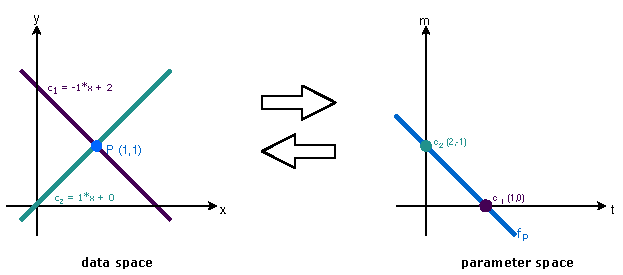
\includegraphics{figures/HoughMXT.pdf}
%     \caption{Caption}
%     \label{fig:houghmxt}
% \end{figure}\todor{eher keine bilder in related work}

\section{CASH}\label{sec:cashintro}
The global correlation clustering algorithm \gls{cash} extends the use case of the Hough Transformation to the detection of arbitrary-dimensional subspaces by augmenting the initial rigid 2-dimensional definition to a multi-dimensional one. 

Furthermore \gls{cash} introduces a improved search strategy for detecting regions of high intersections in parameter space to improve the efficiency compared to the basic grid search \cite{CASHachtert2008global}. Instead of doing an extensive count operation/accumulation of intersections over a fixed interval, \gls{cash} successively splits the whole parameter space by its axes and only further evaluates the split hypercuboids if they contain enough intersections. This is repeated until a certain count of splits is reached and only then hypercuboids with enough intersections are considered as linear correlations. 

Since our work focuses on ``\textit{Detecting Global Correlated Clusters using Hough Transform through Locally Dense Correlations}'', we use \gls{cash} to cope with multi-dimensional data and detect our locally dense correlations. Additionally we will use \gls{cash} as a performance baseline for our descendant algorithm to compare them in a global setting.
A more profound explanation to the transformation and its usage in \gls{cash} will be given in \autoref{ssec:houghindepth}.

% Please add the following required packages to your document preamble:
% \usepackage{booktabs}
% \usepackage{graphicx}
\begin{table}[]
\centering
\resizebox{\textwidth}{!}{%
\begin{tabular}{@{}|l|c|c|c|l|@{}}
\toprule
\textbf{Algorithm}                 & \textbf{\begin{tabular}[c]{@{}c@{}}Local \\ Subspaces\end{tabular}} & \textbf{\begin{tabular}[c]{@{}c@{}}Global \\ Subspaces\end{tabular}} & \textbf{\begin{tabular}[c]{@{}c@{}}Global \\ Subspaces\end{tabular}} & \textbf{Notes}                                                                                                                                                                                                   \\ \midrule
\acrshort{pca}    & \xmark    & \cmark     & \xmark      & \tabitem Only handles single or orthogonal correlations well                                                                                                                                                              \\ \midrule
\acrshort{orclus} & \cmark    & \xmark     & \xmark      & \tabitem Combines \acrshort{pca} with a $k$-Means-like approach                                                                                                                                          \\ \midrule
\acrshort{4c}     & \cmark    & \xmark     & \xmark      & \tabitem Combines \acrshort{pca} with a density-based approach                                                                                                                                           \\ \midrule
\acrshort{copac}  & \xmark    & \cmark     & \xmark      & \begin{tabular}[c]{@{}l@{}}\tabitem Similar to \acrshort{4c}\\ \tabitem Combines \acrshort{pca} with a density-based approach\end{tabular}                                                       \\ \midrule
\acrshort{hico}   & \xmark    & \cmark     & \cmark      & \begin{tabular}[c]{@{}l@{}}\tabitem Creates a Correlation distance ordering similar to \acrshort{optics},\\ \tabitem creates a tree-like hierarchy\end{tabular}                                                   \\ \midrule
\acrshort{eric}   & \xmark    & \cmark     & \cmark      & \begin{tabular}[c]{@{}l@{}}\tabitem Similar to \acrshort{hico}\\ \tabitem Creates a Correlation distance ordering similar to \acrshort{optics}, \\ \quad \ but creates a graph-like hierarchy\end{tabular} \\ \midrule
\acrshort{cash}   & \xmark    & \cmark     & \cmark      & \tabitem Uses the Hough-Transform to                                                                                                                                                                                      \\ \bottomrule
\end{tabular}%
}
\caption{}
\label{tab:corrcluchar}
\end{table}

\section{DBSCAN}\label{sec:dbscanintro}
\citeauthor{DBSCANEKSX96} created a foundational algorithm with \gls{dbscan}. With over 16000 citations on google scholar as of December 2019 it is one of the most influential works created in the field of density-based clustering and a basis to many clustering approaches, not only restricted to density-based clustering. 

As its name reveals it is an algorithm which detects points in dense vicinity and groups them together. For a measure of density \gls{dbscan} utilizes two parameters. One to specify the minimum amount of neighboring points in a close vicinity and one to specify the range/radius of that vicinity. Points fulfilling these conditions are called \textit{core points} and represent the dense \textit{core} of a cluster. The border of a dense cluster is composed of \textit{border points}. They are points which themselves do not possess a dense neighborhood but are still in the vicinity of core points. 

In contrast to $k$-means-like partitioning clustering\cite{kmeansmacqueen1967some}, \gls{dbscan} is able to find not only non-convex shapes, but also any arbitrary shape of a particular density. Since these arbitrary shaped clusters preserves their correlations and our goal is the assembly of locally dense correlations to global correlations, we expect to obtain good results by partitioning our data space via a density-based algorithm.

\section{OPTICS}\label{sec:OPTICSintro}
A disadvantage of \gls{dbscan} is its dependence on a fixed global parameter setting defining the \textit{minimal} detectable density. Assuming a global linear correlation to have low fluctuations in variance and different global linear correlations having various other variances\todor{can i assume this? i have to do some assumptions right?}, finding clusters with single densities would be more advantageous to our algorithm. We therefore adopted the use of \gls{optics} instead, an improvement/extension of \gls{dbscan}, which enables us to extract single densities more accurately \cite{opticsankerst1999optics}. Since \gls{dbscan} and \gls{optics} are the foundations of the partitioning step we will give a more comprehensive explanations to those two algorithms as well (c.f. \autoref{ssec:DBSCANindepth} and \autoref{ssec:OPTICSindepth}).
% Maybe OPTICS? DIRECTLY COPIED OUT OF \cite{ankerst1999optics}
%  First, almost all clustering algorithms require values for input parameters which are hard to
% determine, especially for real-world data sets containing highdimensional objects. Second, the algorithms are very sensible to
% these parameter values, often producing very different partitionings of the data set even for slightly different parameter settings.
% Third, high-dimensional real-data sets often have a very skewed
% distribution that cannot be revealed by a clustering algorithm using only one global parameter setting. 

% \section{Current Optimization Approaches}
% (D-MASC\cite{kazempour2018d, kazempour2019galaxy}, A Galaxy of Correlations etc.) [0.5] \todor{DMASC ist eigtl nur related work zu CASH aber relevant fuer uns?}
    
